\question Q4\droppoints

\begin{solution}
(a)
    Implemented.

    (b) Implemented.

    (c) Implemented.

    (d) Implemented.

    (e) Implemented.

    (f) Implemented.

    (g) Implemented.

    (h) Implemented.

    (i) Implemented.
    The four plots are as follows:

    \centerline{
        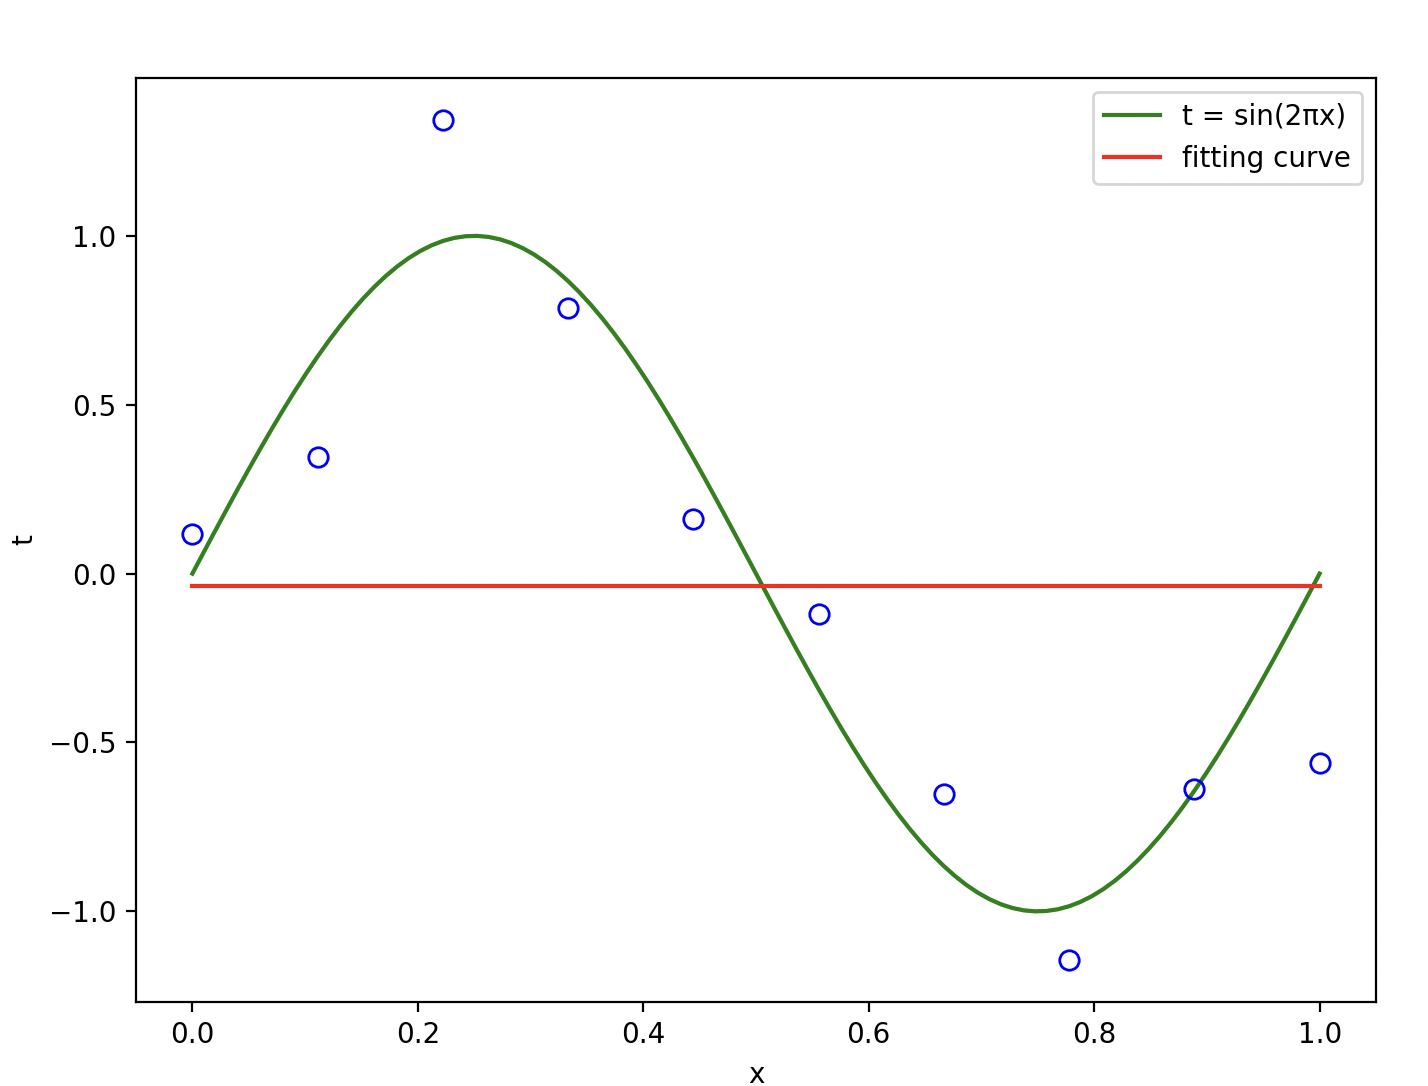
\includegraphics[width=0.75\textwidth]{img/1}
    }
    \centerline{
        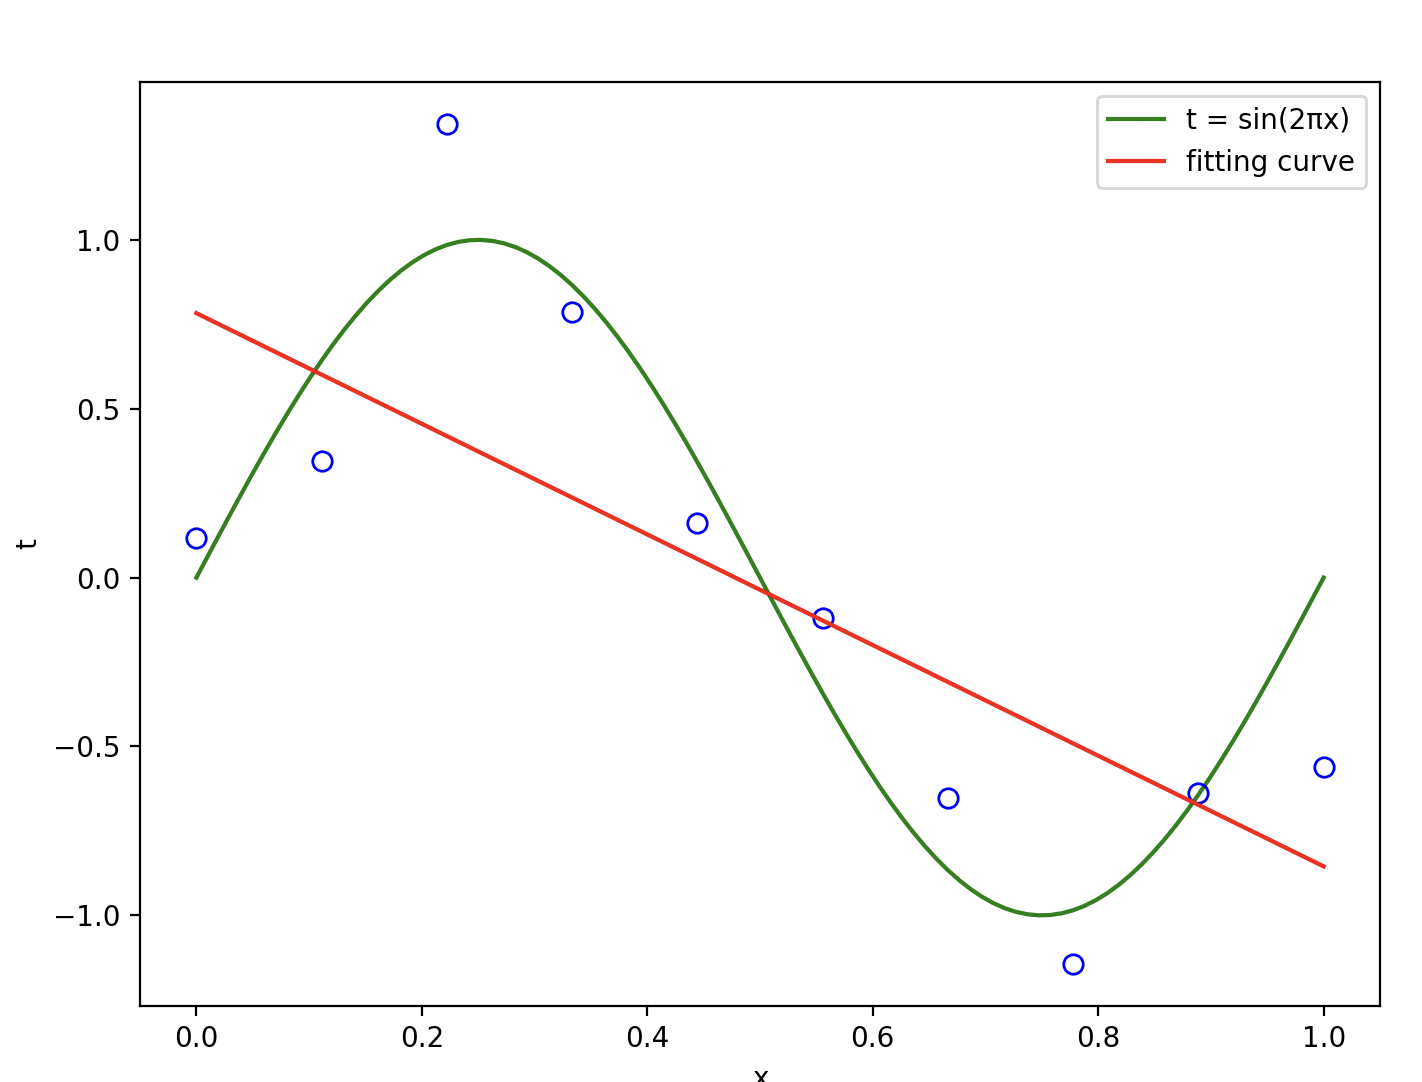
\includegraphics[width=0.75\textwidth]{img/2}
    }
    \centerline{
        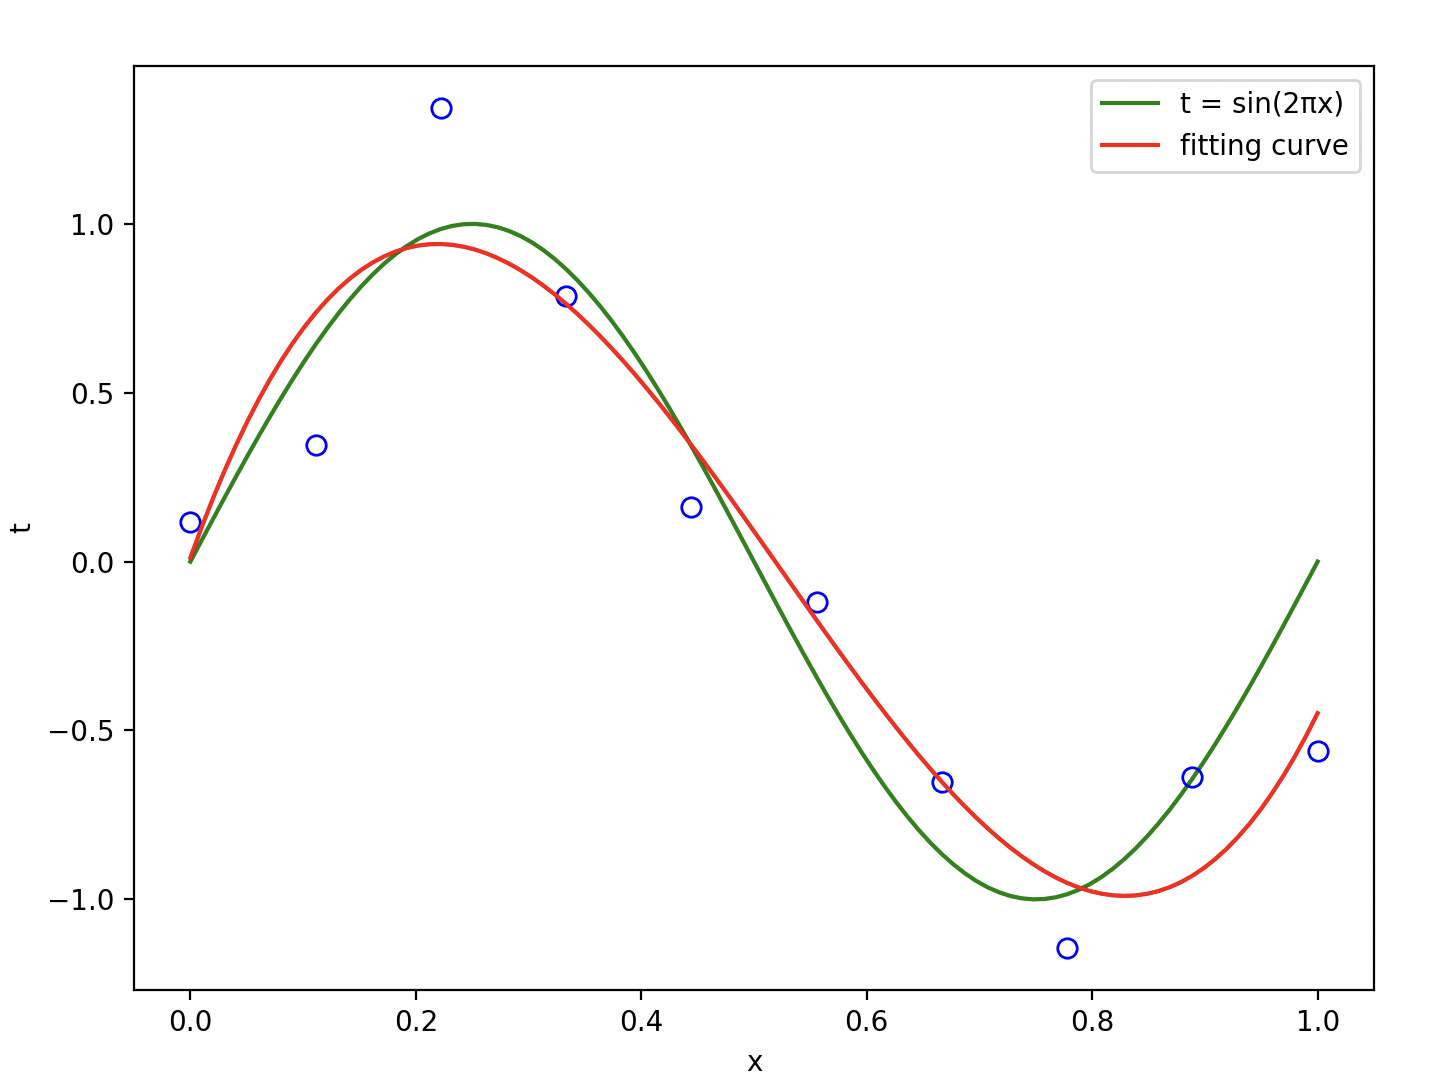
\includegraphics[width=0.75\textwidth]{img/3}
    }
    \centerline{
        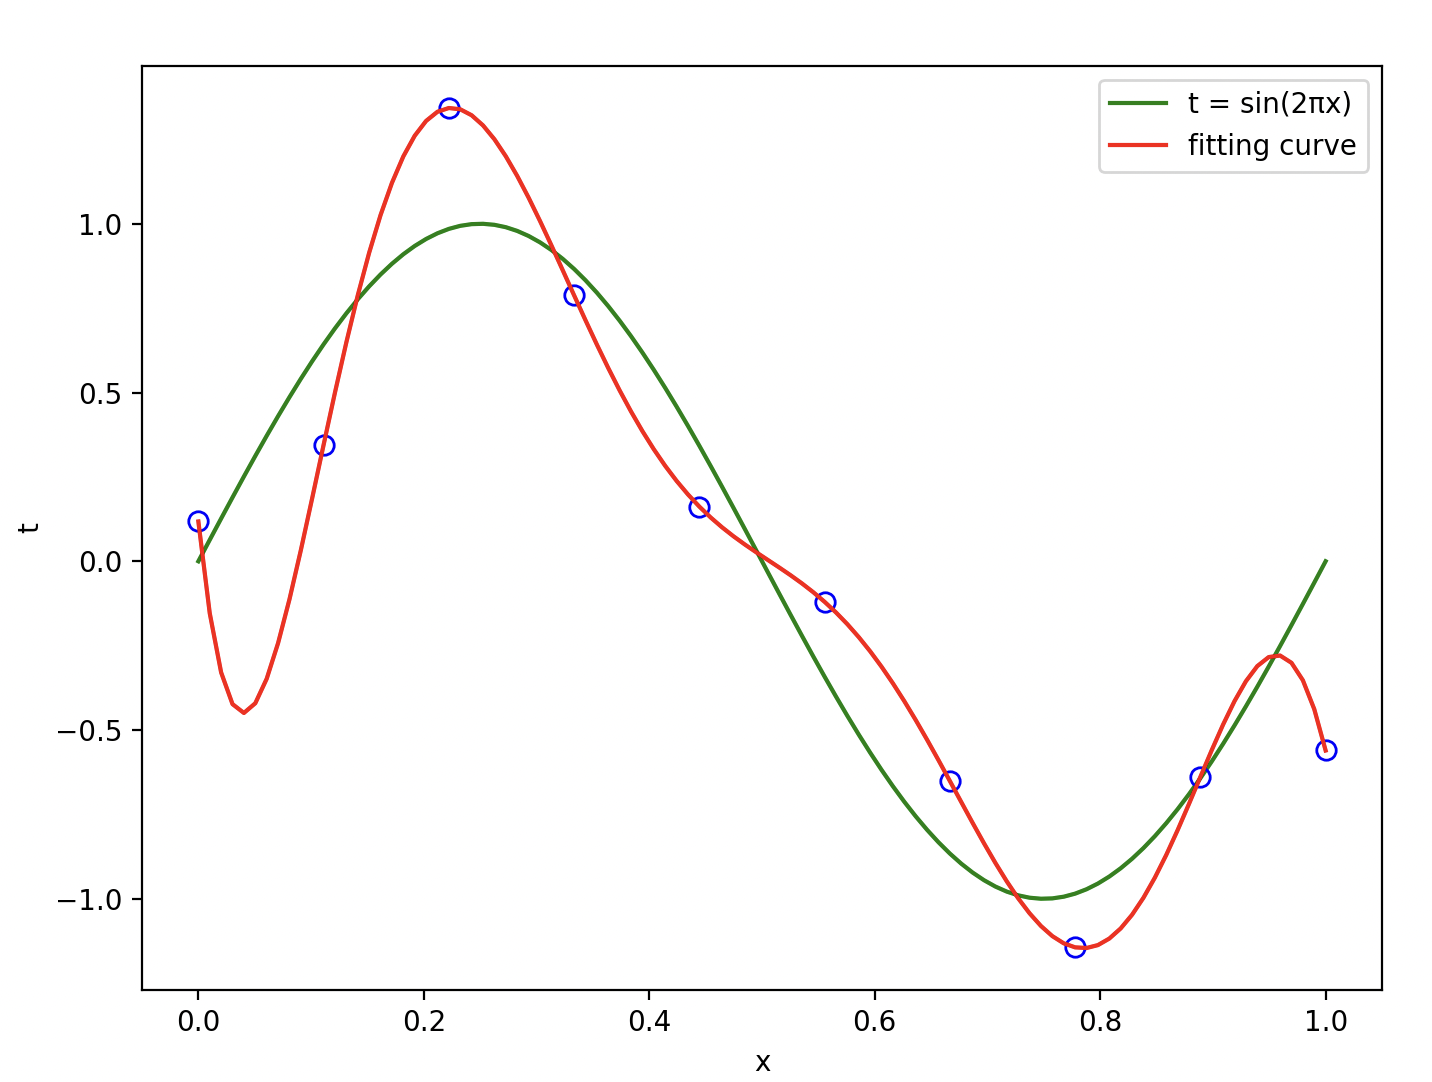
\includegraphics[width=0.75\textwidth]{img/4}
    }

    (j) Implemented.

    (k) Implemented.
    The plot that looks like Figure 1.5 is as follows:

    \centerline{
        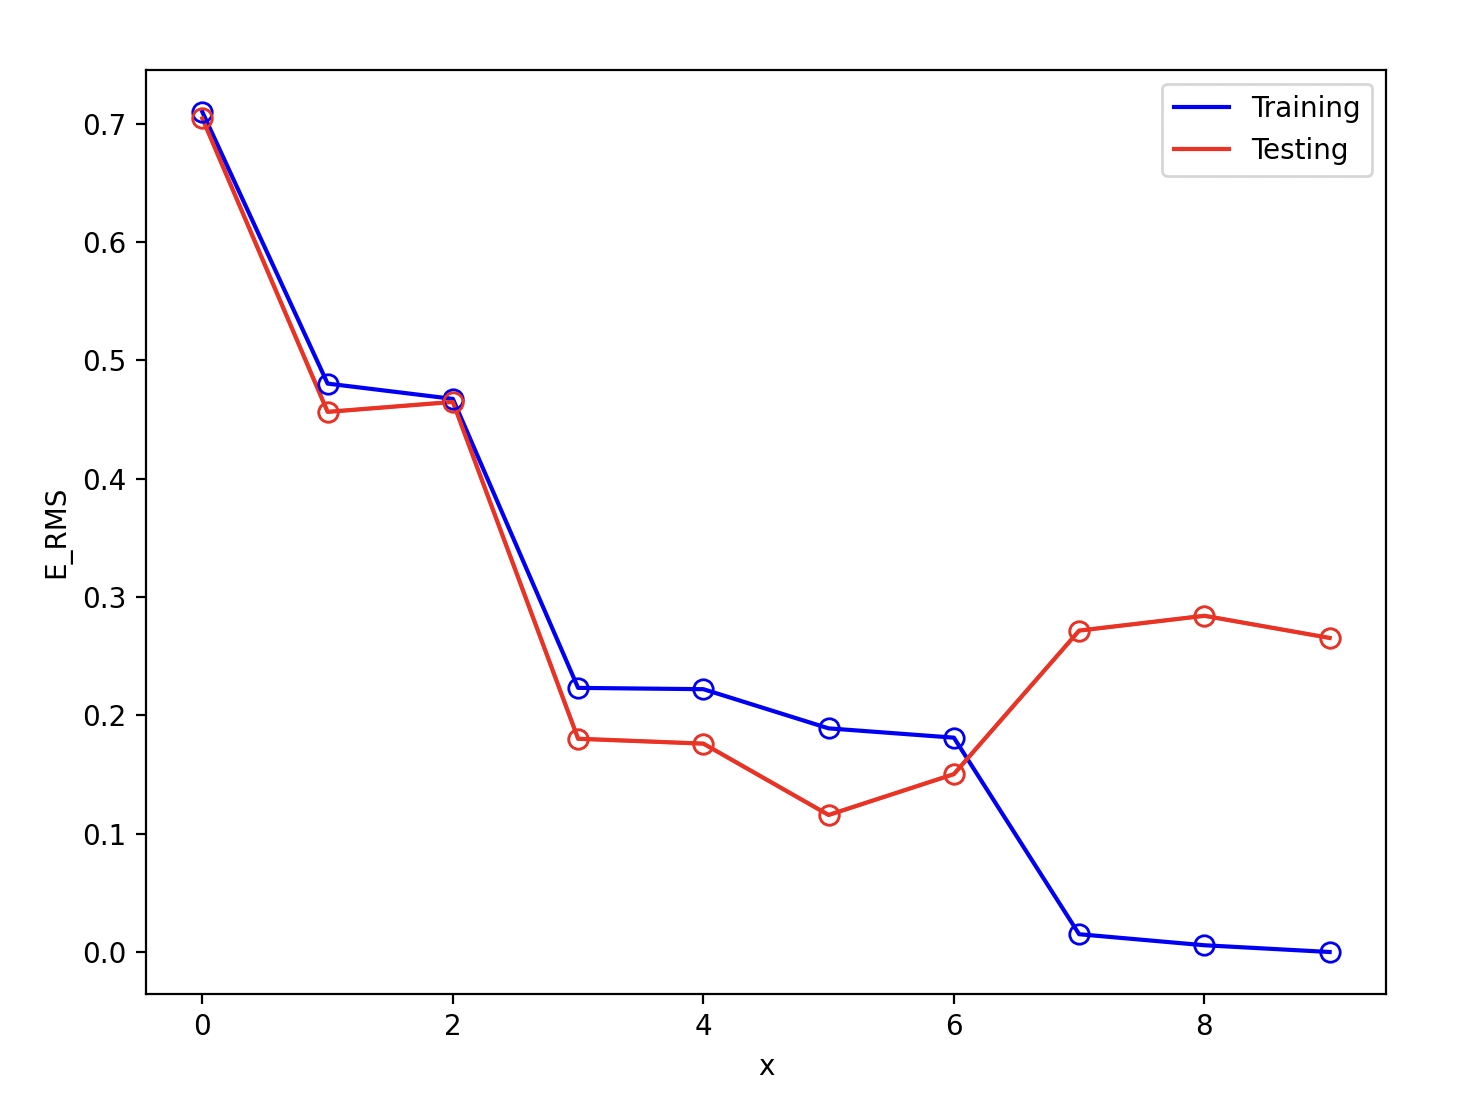
\includegraphics[width=0.75\textwidth]{img/rmse}
    }

    (l) The table is as follows:

    \begin{tabular}{r|rrrrrrrrrr}
        w/M     & 0     & 1     & 2     & 3      & 4      & 5       & 6       & 7         & 8         & 9         \\
        \hline
        $w^*_0$ & -0.04 & 0.78  & 0.6   & 0.01   & -0.01  & 0.07    & 0.09    & 0.12      & 0.12      & 0.12      \\
        $w^*_1$ &       & -1.64 & -0.4  & 9.29   & 10.17  & 2.95    & -2.36   & -34.89    & -40.77    & -32.23    \\
        $w^*_2$ &       &       & -1.23 & -26.79 & -31.24 & 28.96   & 94.52   & 631.3     & 749.85    & 552.58    \\
        $w^*_3$ &       &       &       & 17.04  & 24.17  & -145.98 & -428.17 & -3611.33  & -4505.52  & -2728.57  \\
        $w^*_4$ &       &       &       &        & -3.57  & 191.46  & 736.8   & 9737.36   & 13110.66  & 4762.78   \\
        $w^*_5$ &       &       &       &        &        & -78.01  & -563.1  & -13688.54 & -20711.42 & 2031.29   \\
        $w^*_6$ &       &       &       &        &        &         & 161.69  & 9686.91   & 17880.28  & -19359.54 \\
        $w^*_7$ &       &       &       &        &        &         &         & -2721.49  & -7737.84  & 28382.47  \\
        $w^*_8$ &       &       &       &        &        &         &         &           & 1254.09   & -17856.18 \\
        $w^*_9$ &       &       &       &        &        &         &         &           &           & 4246.73
    \end{tabular}

    (m) According to the results in part (j), the order $5$ would be the best for this data set, as it results in the least root-mean-square error for testing set.

    (n)
    \begin{enumerate}
        \item {
            \textbf{Sensitive to Outliers}: An outlier will increase the error dramatically, resulting in a terrible fitting. To avoid this, we can pre-process the training data set and remove the outliers first.
        }
        \item {
            \textbf{Overfitting Problem}: The least square approach can easily lead to overfitting when the order of polynomial is too large. We can address this by selecting a proper order.
        }
    \end{enumerate}

\end{solution}